%\documentclass[portrait,final,a0paper]{baposter}
\documentclass[a0paper,portrait,final]{baposter}
% Usa a4shrink for an a4 sized paper.

\tracingstats=2

\usepackage{calc}
\usepackage{graphicx}
\usepackage{amsmath}
\usepackage{amssymb}
\usepackage{relsize}
\usepackage{multirow}
\usepackage{bm}

\usepackage{graphicx}
\usepackage{scalefnt}
\usepackage{multicol}
\usepackage{footmisc}

\usepackage{pgfbaselayers}
\pgfdeclarelayer{background}
\pgfdeclarelayer{foreground}
\pgfsetlayers{background,main,foreground}

\usepackage{times}
\usepackage{helvet}
%\usepackage{bookman}
\usepackage{palatino}


\newcommand{\captionfont}{\footnotesize}

%\renewcommand{\thefootnote}{\roman{footnote}}
\selectcolormodel{cmyk}

\graphicspath{{images/}}


%%%%%%%%%%%%%%%%%%%%%%%%%%%%%%%%%%%%%%%%%%%%%%%%%%%%%%%%%%%%%%%%%%%%%%%%%%%%%%%%
%%%% Some math symbols used in the text
%%%%%%%%%%%%%%%%%%%%%%%%%%%%%%%%%%%%%%%%%%%%%%%%%%%%%%%%%%%%%%%%%%%%%%%%%%%%%%%%
% Format 
\newcommand{\Matrix}[1]{\begin{bmatrix} #1 \end{bmatrix}}
\newcommand{\Vector}[1]{\Matrix{#1}}
\newcommand*{\SET}[1]  {\ensuremath{\mathcal{#1}}}
\newcommand*{\MAT}[1]  {\ensuremath{\mathbf{#1}}}
\newcommand*{\VEC}[1]  {\ensuremath{\bm{#1}}}
\newcommand*{\CONST}[1]{\ensuremath{\mathit{#1}}}
\newcommand*{\norm}[1]{\mathopen\| #1 \mathclose\|}% use instead of $\|x\|$
\newcommand*{\abs}[1]{\mathopen| #1 \mathclose|}% use instead of $\|x\|$
\newcommand*{\absLR}[1]{\left| #1 \right|}% use instead of $\|x\|$

\def\norm#1{\mathopen\| #1 \mathclose\|}% use instead of $\|x\|$
\newcommand{\normLR}[1]{\left\| #1 \right\|}% use instead of $\|x\|$

%%%%%%%%%%%%%%%%%%%%%%%%%%%%%%%%%%%%%%%%%%%%%%%%%%%%%%%%%%%%%%%%%%%%%%%%%%%%%%%%
% Multicol Settings
%%%%%%%%%%%%%%%%%%%%%%%%%%%%%%%%%%%%%%%%%%%%%%%%%%%%%%%%%%%%%%%%%%%%%%%%%%%%%%%%
\setlength{\columnsep}{1.1em}
\setlength{\columnseprule}{0.0mm}


%%%%%%%%%%%%%%%%%%%%%%%%%%%%%%%%%%%%%%%%%%%%%%%%%%%%%%%%%%%%%%%%%%%%%%%%%%%%%%%%
% Save space in lists. Use this after the opening of the list
%%%%%%%%%%%%%%%%%%%%%%%%%%%%%%%%%%%%%%%%%%%%%%%%%%%%%%%%%%%%%%%%%%%%%%%%%%%%%%%%
\newcommand{\compresslist}{%
\setlength{\itemsep}{0.1em}%
\setlength{\parskip}{0.0pt}%
\setlength{\parsep}{0.0pt}%
}


%%%%%%%%%%%%%%%%%%%%%%%%%%%%%%%%%%%%%%%%%%%%%%%%%%%%%%%%%%%%%%%%%%%%%%%%%%%%%%
%%% Begin of Document
%%%%%%%%%%%%%%%%%%%%%%%%%%%%%%%%%%%%%%%%%%%%%%%%%%%%%%%%%%%%%%%%%%%%%%%%%%%%%%

\begin{document}
\def\@xfootnote[#1]{%
  \protected@xdef\@thefnmark{#1}%
  \@footnotemark\@footnotetext}

%\renewcommand{\thefootnote}{\roman{footnote}}
%\renewcommand{\thefootnote}{$^{\it \roman{footnote}}$}

%%%%%%%%%%%%%%%%%%%%%%%%%%%%%%%%%%%%%%%%%%%%%%%%%%%%%%%%%%%%%%%%%%%%%%%%%%%%%%
%%% Here starts the poster
%%%---------------------------------------------------------------------------
%%% Format it to your taste with the options
%%%%%%%%%%%%%%%%%%%%%%%%%%%%%%%%%%%%%%%%%%%%%%%%%%%%%%%%%%%%%%%%%%%%%%%%%%%%%%
% Define some colors
\definecolor{silver}{cmyk}{0,0,0,0.3}
%\definecolor{coral}{cmyk}{0,0.5,0.69,0.0}
\definecolor{coral}{cmyk}{0,0.58,0.69,0.0}
\definecolor{lightcoral}{cmyk}{0,0.48,0.59,0.0}
\definecolor{black}{cmyk}{0,0,0.0,1.0}
\definecolor{red}{rgb}{1,0,0}
\definecolor{darkYellow}{cmyk}{0,0,1.0,0.5}
\definecolor{darkSilver}{cmyk}{0,0,0,0.1}
\definecolor{darksalmon}{cmyk}{0,0.36,0.48,0.09}
\definecolor{salmon5}{cmyk}{0,0.41,0.41,0.56}

\definecolor{lightercoral}{cmyk}{0,0.25,0.25,0}
%\definecolor{lightercoral}{cmyk}{0,0.40,0.47,0.08}
\definecolor{apricot}{cmyk}{0.0,0.36,0.57,0.02}
\definecolor{lightestapricot}{cmyk}{0,0,0.05,0.0}

%%
\typeout{Poster Starts}
%\background{
%  \begin{tikzpicture}[remember picture,overlay]%
    %\draw (current page.north west)+(-2em,2em) node[anchor=north west] {\includegraphics[height=1.1\textheight]{silhouettes_background}};

%  \end{tikzpicture}%
%}

\newlength{\leftimgwidth}
\begin{poster}%
  % Poster Options
  {
  % Show grid to help with alignment
  grid=no,
  % Column spacing
  colspacing=0.5em,
  % Color style
%  bgColorOne=white,
%  bgColorOne=darksalmon,
  bgColorOne=white,
  %bgColorTwo=darksalmon,
  bgColorTwo=white,
  %bgColorThree=red,
  borderColor=red,
  %headerColorOne=white,
  headerColorOne=lightcoral,
  headerColorOne=white,
  headerColorTwo=darksalmon,
  headerColorTwo=white,
  headerFontColor=black,
  boxColorOne=lightercoral,
  boxColorOne=white,
  boxColorTwo=lightercoral,
  % Format of textbox
  textborder=roundedleft,
  %textborder=rectangle,
  % Format of text header
  eyecatcher=yes,
  headerborder=closed,
  headerheight=0.08\textheight,
  headershape=roundedright,
  headershade=shade-tb,
  headerfont=\Large\textsf, %Sans Serif
  boxshade=plain,
  textfont={\sf },
  background=shade-tb,
  %background=plain,
  linewidth=1pt,
  columns=4
  }
  {
    \makebox[15em][l]{%
      %\begin{minipage}{8em}
        \includegraphics[height=.085\textwidth]{acm.eps}
      %\end{minipage} 
    }
   }
  {\sc V4VSockets}
  { \sc\vspace{0.5em} low overhead intra-node communication in Xen}
  {   \makebox[15em][r]{%
      \begin{minipage}{14.5em}
        %\vfill
        \includegraphics[height=4.5em]{cslab_logo.pdf}
       \end{minipage}}
    %\makebox[5em][r]{% \includegraphics[height=5.0em]{ntua_logo.pdf} }
   }

%%%%%%%%%%%%%%%%%%%%%%%%%%%%%%%%%%%%%%%%%%%%%%%%%%%%%%%%%%%%%%%%%%%%%%%%%%%%%%
%  \headerbox{Motivation}{name=motivation,column=0,row=0, span=1}{
%%%%%%%%%%%%%%%%%%%%%%%%%%%%%%%%%%%%%%%%%%%%%%%%%%%%%%%%%%%%%%%%%%%%%%%%%%%%%%

%Intra-node communication suffers from severe overheads mostly due to:
%\begin{itemize}
%\item inefficient data paths
%\item packet handling
%\end{itemize}
%}
%%%%%%%%%%%%%%%%%%%%%%%%%%%%%%%%%%%%%%%%%%%%%%%%%%%%%%%%%%%%%%%%%%%%%%%%%%%%%%%
 \headerbox{I/O Path in Xen (generic environment)}{name=xenpath,row=0,column=0, span=2}{
%%%%%%%%%%%%%%%%%%%%%%%%%%%%%%%%%%%%%%%%%%%%%%%%%%%%%%%%%%%%%%%%%%%%%%%%%%%%%%%
%\begin{multicols}{2}

%\hspace{0.5em}
%\begin{figure}
\begin{center}
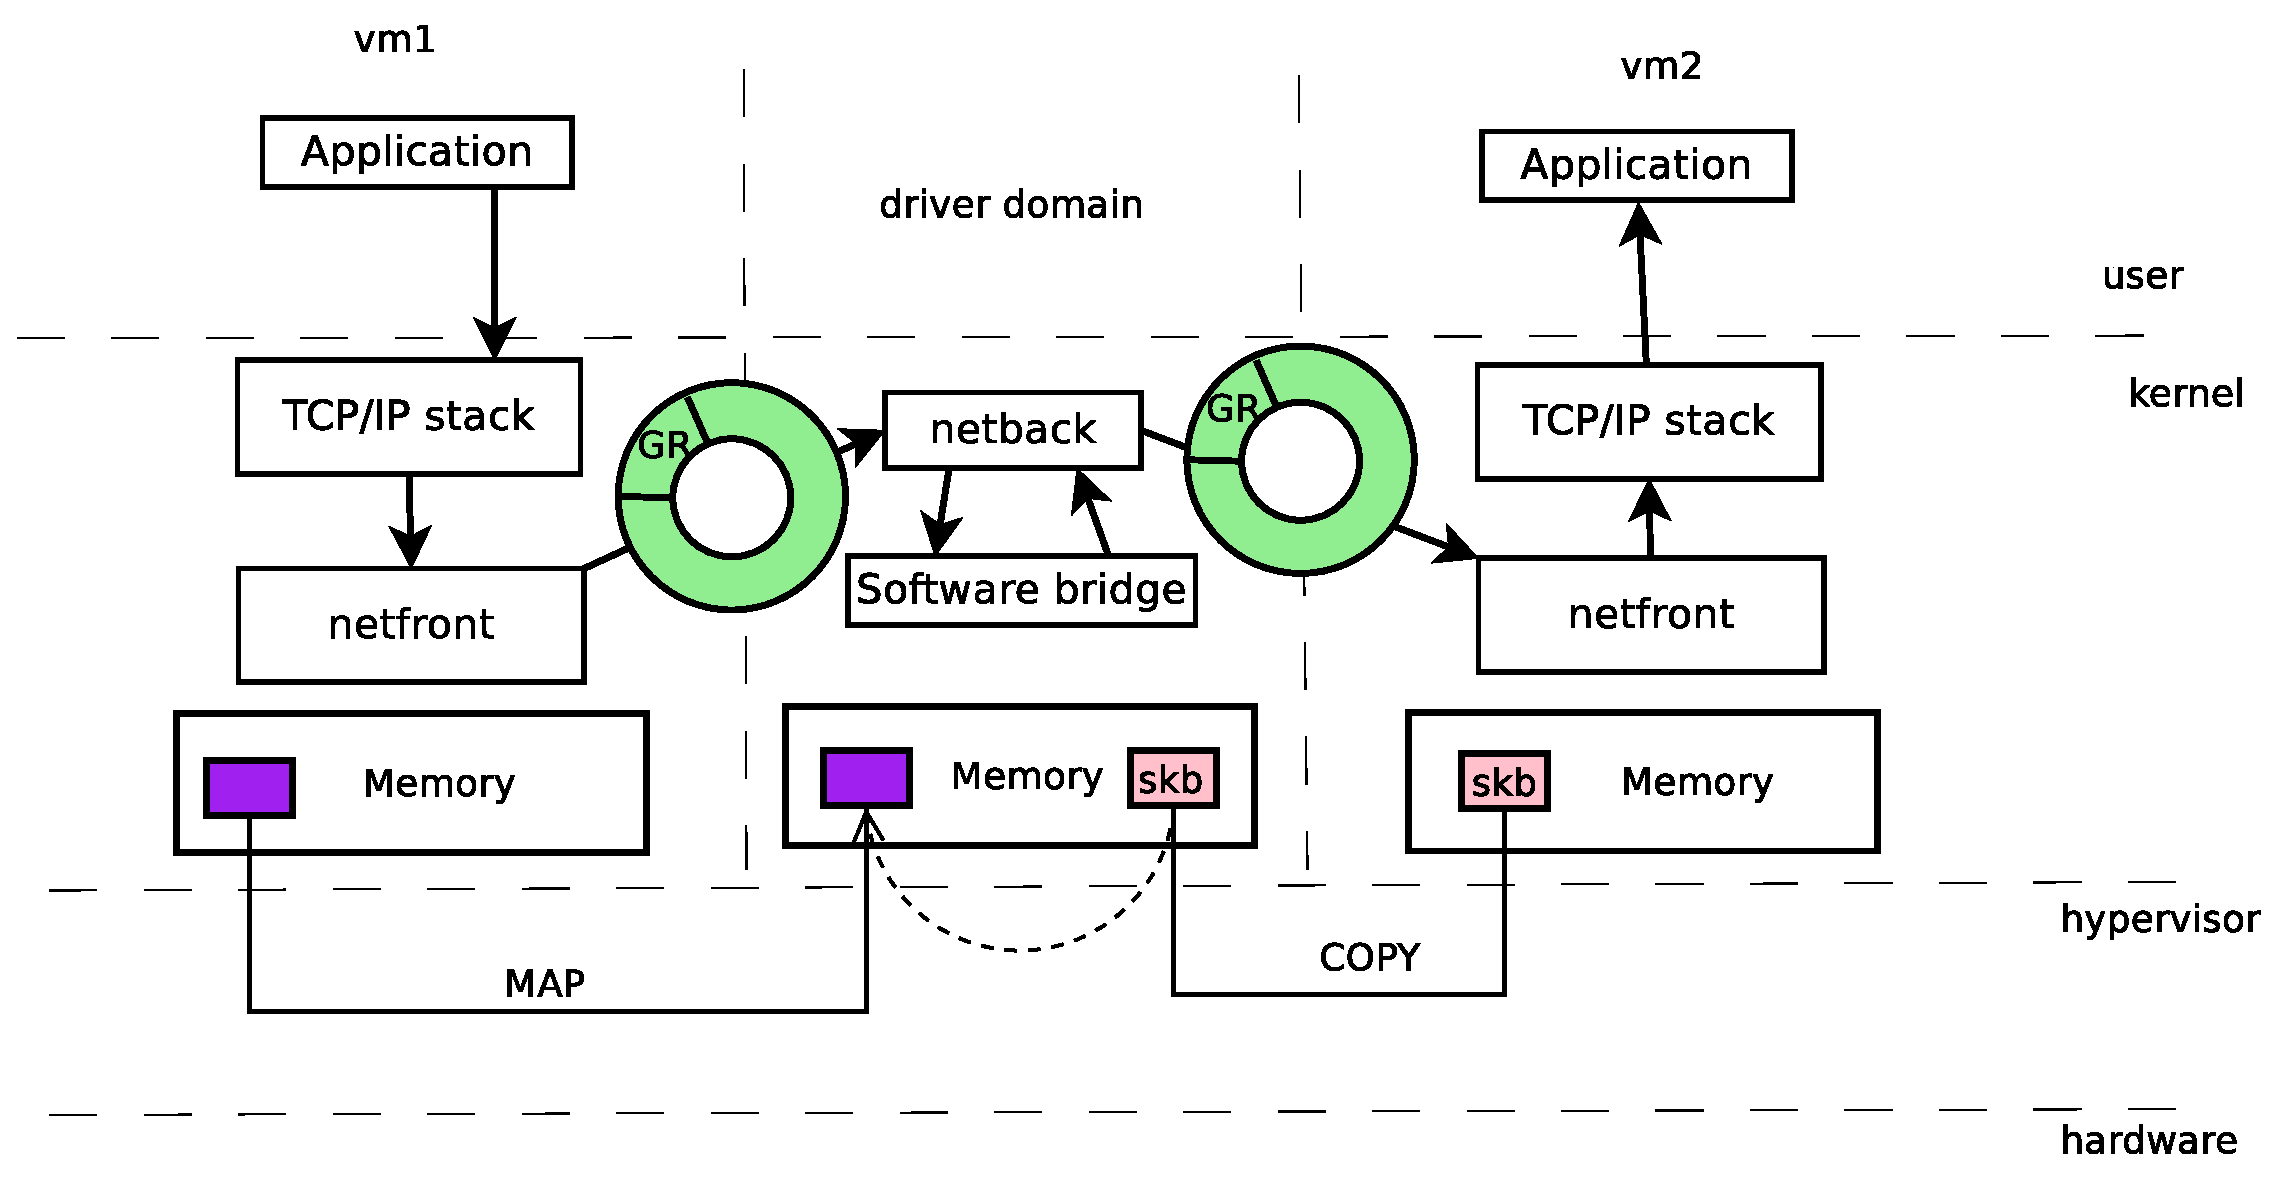
\includegraphics[width=.9\linewidth]{figures/netfront_netback.eps}
\end{center}
%\end{figure}
Intra-node communication suffers from severe overheads:
%\begin{multicols}{2}
%\setlength{\columnsep}{0.3em}
%\setlength{\columnseprule}{0.0mm}

\begin{itemize}
\compresslist
\item[$\Rightarrow$] inefficient data paths

\item[$\Rightarrow$] driver domain handles packet forwarding

\item[$\Rightarrow$] unnecessary TCP/IP stack crossing and fragmentation

\end{itemize}
%\end{multicols}
\vspace{0.5em}

}

\headerbox{I/O Path in Xen with V4VSockets}{name=v4vpath,row=0,column=2, span=2}{
%\hspace{0.5em}\scalebox{.96}{
\begin{center}
\includegraphics[width=.9\linewidth]{figures/v4vsockets.eps}
\end{center}
%}
%\includegraphics[width=.5\linewidth]{}
%layer and use the hypervisor as the control \emph{and} the data plane. 

V4VSockets is built as a full-stack protocol framework that supports
p2p communication between VMs. %We bypass the intermediate

%\begin{multicols}{2}
%\setlength{\columnsep}{0.3em}
\begin{flushleft}
\begin{itemize}
\compresslist
\item[$\Rightarrow$] \emph{Application layer}: the socket interface.

\item[$\Rightarrow$] \emph{Transport layer}: VM kernel driver.

\item[$\Rightarrow$] \emph{Network/Link layer}: the hypervisor, providing encapsulation of upper-layer messages to V4V messages, and packet delivery.

\end{itemize}
\end{flushleft}
%\end{multicols}
\vspace{.5em}
}

%%%%%%%%%%%%%%%%%%%%%%%%%%%%%%%%%%%%%%%%%%%%%%%%%%%%%%%%%%%%%%%%%%%%%%%%%%%%%%
  \headerbox{Key features}{name=contribution,column=0,span=2, below=xenpath}{
%%%%%%%%%%%%%%%%%%%%%%%%%%%%%%%%%%%%%%%%%%%%%%%%%%%%%%%%%%%%%%%%%%%%%%%%%%%%%%
V4VSockets is an efficient, socket-compliant, high performance intra node communication framework.
\vspace{.5em}

V4VSockets features:
\begin{flushleft}
\begin{itemize}
\compresslist
\item[$\Rightarrow$] \emph{optimized data path} (data are copied from~/~to the VM kernel memory without the need to share pages between VMs)

\item[$\Rightarrow$] \emph{low-overhead} framework (no intermediary VM --
driver domain -- no scheduling implications are involved) 

\item[$\Rightarrow$] \emph{secure} (no security implications -- data cross the hypervisor and either get dropped or pushed forward using V4V semantics)
\item[$\Rightarrow$] \emph{ultra low latency} and \emph{high bandwidth}
\item[$\Rightarrow$] Open-source, available @ \texttt{https://github.com/HPSI/v4v}
\end{itemize}
\end{flushleft}

\vspace{.5em}
}


%%%%%%%%%%%%%%%%%%%%%%%%%%%%%%%%%%%%%%%%%%%%%%%%%%%%%%%%%%%%%%%%%%%%%%%%%%%%%%%%
%% \headerbox{Acknowledgements}{name=acknowledgements,column=0,above=bottom}{
%%%%%%%%%%%%%%%%%%%%%%%%%%%%%%%%%%%%%%%%%%%%%%%%%%%%%%%%%%%%%%%%%%%%%%%%%%%%%%%%
%%  \small
%%%  \hspace{1em}
%%   The authors would like to thank Nikos Nikoleris, Elisavet Kozyri and Stratos Psomadakis for their usefull contributions to this work.
%%\vspace{0.5em}
%%  }
%
%%%%%%%%%%%%%%%%%%%%%%%%%%%%%%%%%%%%%%%%%%%%%%%%%%%%%%%%%%%%%%%%%%%%%%%%%%%%%%%
\headerbox{Ping-pong benchmark on 2x Xeon X5650, 48 GB}{name=results,column=2,span=2,below=v4vpath}{

\setlength{\columnsep}{0em}
%\setlength{\columnseprule}{0.9mm}
\begin{multicols}{2}

\hspace{0.0em}\scalebox{.95}{
\includegraphics[width=\linewidth]{figures/v4v_lat.eps}}

\hspace{0.0em}\scalebox{.95}{
\includegraphics[width=\linewidth]{figures/v4v_bw.eps}}

\end{multicols}
\begin{center}
\scalebox{.870}{
\includegraphics[width=\linewidth]{figures/new_stream_bw_scale.eps}}
\end{center}

\vspace {-1em}
V4VSockets:
\begin{itemize}
\compresslist
\item[$\Rightarrow$] improves latency for small messages by 81\% 
\item[$\Rightarrow$] achieves 2299 MB/s for large messages (1 MB) vs. 501 MB/s
\item[$\Rightarrow$] scales efficiently with the number of VMs, both in terms of latency and bandwidth
\item[$\Rightarrow$] achieves aggregate throughput $\approx$ 17 GB/s for 512 KB messages when 16 VMs exchange data in pairs
\end{itemize}

 %bringing memory-copy-like bandwidth measurements to VM--to--VM message exchange.

%\end{multicols}

}

\headerbox{GPU stencil performance through rCUDA}{name=gpu,column=0,span=2,below=contribution}{
\begin{multicols}{2} 

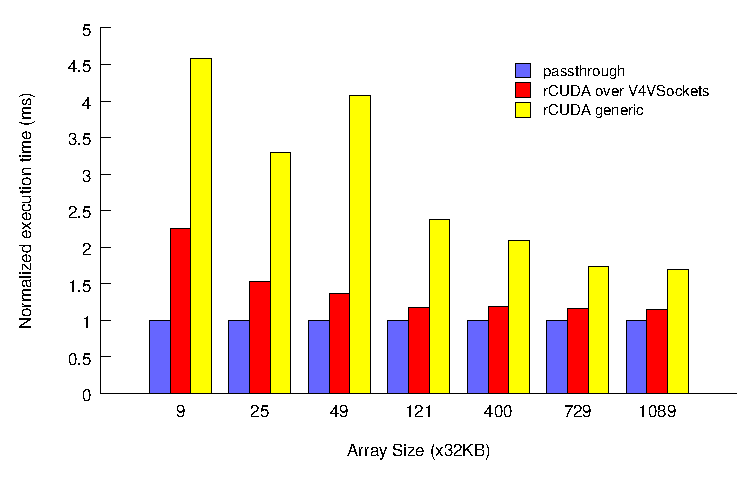
\includegraphics[width=\linewidth]{figures/total_cublas_time.eps}
\scalebox{0.89}{
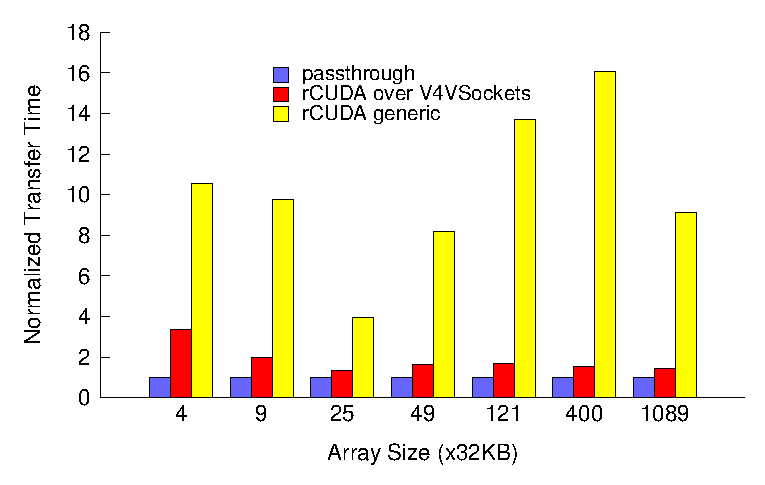
\includegraphics[width=\linewidth]{figures/matrixA_cublas_throughput.eps}
}
\end{multicols}

We run the matrix-matrix product benchmark: (a) natively via GPU passthrough, (b) via rCUDA over TCP/IP sockets and (c) via rCUDA over V4VSockets. Steps include: (i) 2x input matrix copies, (ii) GPU product compute, (iii) 1x output matrix copy back. V4VSockets:
\begin{itemize}
\compresslist
%\item[$\Rightarrow$] matrix-matrix product benchmark run: (a) natively via GPU passthrough, (b) rCUDA over TCP/IP sockets and (c) rCUDA over V4VSockets
%\item[$\Rightarrow$] steps: 2x matrix copy, GPU compute, 1x copy back.
\item[$\Rightarrow$] adds a minimum overhead of 15\% (compared to native execution)
\item[$\Rightarrow$] boosts transfer throughput by 7x (at best) compared to TCP/IP
\end{itemize}
\vspace{.5em}

%We observe that the peak throughput is 3.79 GB/s in our baseline experiment,
%while the respective throughput in the remote V4VSockets case is 2.46 GB/s.
%However, for a matrix size of 34 MB (2112 x 4224 float type elements)
%V4VSockets outperforms the generic case by a factor of 7 (0.35 GB/s).
%\end{multicols}

%\vspace{1em}
}
\headerbox{\small Contact info and Acknowledgments}{name=acks,column=2,span=2,below=results}{
\scalefont{.85}
\begin{center}
Anastassios Nanos, %\footnote{Currently with OnApp Ltd.}, 
Stefanos Gerangelos, Ioanna Alifieraki
%\footnote{Currently with the University of Manchester} 
and Nectarios Koziris\\
 \{ananos,sgerag,ialif,nkoziris\}@cslab.ece.ntua.gr\\
\texttt{http://www.cslab.ece.ntua.gr/research}
\end{center}

%\begin{multicols}{2}
\begin{minipage}{\linewidth}
%\scalefont{.7}
\footnotesize
%\renewcommand{\baselinestretch}{0.8}
%\renewcommand{\baselineskip}{0.4em}
The authors would like to thank the members of CSLab for the stimulating
conversations that led to this work, especially Dr~George Goumas,
Dr~Konstantinos Nikas and Nikela Papadopoulou. Additionally, many thanks to the
anonymous reviewers for their useful comments and suggestions.
\end{minipage}
%\end{multicols}
\vspace{1em}
}

\headerbox{Work in Progress}{name=wip,column=0,span=2,below=gpu}{
%We plan to:
\begin{itemize}
\compresslist
\item[$\Rightarrow$] Strengthen our implementation towards a more user-friendly approach.
\item[$\Rightarrow$] Thoroughly examine the CPU utilization overheads imposed by V4VSockets. 
\item[$\Rightarrow$] Polish the peer discovery framework to adaptively use V4VSockets over generic sockets. 
\item[$\Rightarrow$] Perform an elaborate performance evaluation of the GPU sharing framework we have developed.
\end{itemize}


\vspace{.5em}
}
\end{poster}

\end{document}
